% Options for packages loaded elsewhere
\PassOptionsToPackage{unicode}{hyperref}
\PassOptionsToPackage{hyphens}{url}
\PassOptionsToPackage{dvipsnames,svgnames,x11names}{xcolor}
%
\documentclass[
  a4paper,
]{article}
\usepackage{amsmath,amssymb}
\usepackage{iftex}
\ifPDFTeX
  \usepackage[T1]{fontenc}
  \usepackage[utf8]{inputenc}
  \usepackage{textcomp} % provide euro and other symbols
\else % if luatex or xetex
  \usepackage{unicode-math} % this also loads fontspec
  \defaultfontfeatures{Scale=MatchLowercase}
  \defaultfontfeatures[\rmfamily]{Ligatures=TeX,Scale=1}
\fi
\usepackage{lmodern}
\ifPDFTeX\else
  % xetex/luatex font selection
\fi
% Use upquote if available, for straight quotes in verbatim environments
\IfFileExists{upquote.sty}{\usepackage{upquote}}{}
\IfFileExists{microtype.sty}{% use microtype if available
  \usepackage[]{microtype}
  \UseMicrotypeSet[protrusion]{basicmath} % disable protrusion for tt fonts
}{}
\makeatletter
\@ifundefined{KOMAClassName}{% if non-KOMA class
  \IfFileExists{parskip.sty}{%
    \usepackage{parskip}
  }{% else
    \setlength{\parindent}{0pt}
    \setlength{\parskip}{6pt plus 2pt minus 1pt}}
}{% if KOMA class
  \KOMAoptions{parskip=half}}
\makeatother
\usepackage{xcolor}
\usepackage[margin = 2cm]{geometry}
\usepackage{color}
\usepackage{fancyvrb}
\newcommand{\VerbBar}{|}
\newcommand{\VERB}{\Verb[commandchars=\\\{\}]}
\DefineVerbatimEnvironment{Highlighting}{Verbatim}{commandchars=\\\{\}}
% Add ',fontsize=\small' for more characters per line
\usepackage{framed}
\definecolor{shadecolor}{RGB}{248,248,248}
\newenvironment{Shaded}{\begin{snugshade}}{\end{snugshade}}
\newcommand{\AlertTok}[1]{\textcolor[rgb]{0.94,0.16,0.16}{#1}}
\newcommand{\AnnotationTok}[1]{\textcolor[rgb]{0.56,0.35,0.01}{\textbf{\textit{#1}}}}
\newcommand{\AttributeTok}[1]{\textcolor[rgb]{0.13,0.29,0.53}{#1}}
\newcommand{\BaseNTok}[1]{\textcolor[rgb]{0.00,0.00,0.81}{#1}}
\newcommand{\BuiltInTok}[1]{#1}
\newcommand{\CharTok}[1]{\textcolor[rgb]{0.31,0.60,0.02}{#1}}
\newcommand{\CommentTok}[1]{\textcolor[rgb]{0.56,0.35,0.01}{\textit{#1}}}
\newcommand{\CommentVarTok}[1]{\textcolor[rgb]{0.56,0.35,0.01}{\textbf{\textit{#1}}}}
\newcommand{\ConstantTok}[1]{\textcolor[rgb]{0.56,0.35,0.01}{#1}}
\newcommand{\ControlFlowTok}[1]{\textcolor[rgb]{0.13,0.29,0.53}{\textbf{#1}}}
\newcommand{\DataTypeTok}[1]{\textcolor[rgb]{0.13,0.29,0.53}{#1}}
\newcommand{\DecValTok}[1]{\textcolor[rgb]{0.00,0.00,0.81}{#1}}
\newcommand{\DocumentationTok}[1]{\textcolor[rgb]{0.56,0.35,0.01}{\textbf{\textit{#1}}}}
\newcommand{\ErrorTok}[1]{\textcolor[rgb]{0.64,0.00,0.00}{\textbf{#1}}}
\newcommand{\ExtensionTok}[1]{#1}
\newcommand{\FloatTok}[1]{\textcolor[rgb]{0.00,0.00,0.81}{#1}}
\newcommand{\FunctionTok}[1]{\textcolor[rgb]{0.13,0.29,0.53}{\textbf{#1}}}
\newcommand{\ImportTok}[1]{#1}
\newcommand{\InformationTok}[1]{\textcolor[rgb]{0.56,0.35,0.01}{\textbf{\textit{#1}}}}
\newcommand{\KeywordTok}[1]{\textcolor[rgb]{0.13,0.29,0.53}{\textbf{#1}}}
\newcommand{\NormalTok}[1]{#1}
\newcommand{\OperatorTok}[1]{\textcolor[rgb]{0.81,0.36,0.00}{\textbf{#1}}}
\newcommand{\OtherTok}[1]{\textcolor[rgb]{0.56,0.35,0.01}{#1}}
\newcommand{\PreprocessorTok}[1]{\textcolor[rgb]{0.56,0.35,0.01}{\textit{#1}}}
\newcommand{\RegionMarkerTok}[1]{#1}
\newcommand{\SpecialCharTok}[1]{\textcolor[rgb]{0.81,0.36,0.00}{\textbf{#1}}}
\newcommand{\SpecialStringTok}[1]{\textcolor[rgb]{0.31,0.60,0.02}{#1}}
\newcommand{\StringTok}[1]{\textcolor[rgb]{0.31,0.60,0.02}{#1}}
\newcommand{\VariableTok}[1]{\textcolor[rgb]{0.00,0.00,0.00}{#1}}
\newcommand{\VerbatimStringTok}[1]{\textcolor[rgb]{0.31,0.60,0.02}{#1}}
\newcommand{\WarningTok}[1]{\textcolor[rgb]{0.56,0.35,0.01}{\textbf{\textit{#1}}}}
\usepackage{graphicx}
\makeatletter
\def\maxwidth{\ifdim\Gin@nat@width>\linewidth\linewidth\else\Gin@nat@width\fi}
\def\maxheight{\ifdim\Gin@nat@height>\textheight\textheight\else\Gin@nat@height\fi}
\makeatother
% Scale images if necessary, so that they will not overflow the page
% margins by default, and it is still possible to overwrite the defaults
% using explicit options in \includegraphics[width, height, ...]{}
\setkeys{Gin}{width=\maxwidth,height=\maxheight,keepaspectratio}
% Set default figure placement to htbp
\makeatletter
\def\fps@figure{htbp}
\makeatother
\setlength{\emergencystretch}{3em} % prevent overfull lines
\providecommand{\tightlist}{%
  \setlength{\itemsep}{0pt}\setlength{\parskip}{0pt}}
\setcounter{secnumdepth}{-\maxdimen} % remove section numbering
\usepackage{fvextra}
\DefineVerbatimEnvironment{Highlighting}{Verbatim}{breaklines,breaksymbolleft={},commandchars=\\\{\}}
\usepackage{tcolorbox}
\usepackage[default]{lato}
\usepackage{booktabs}
\usepackage{longtable}
\usepackage{array}
\usepackage{multirow}
\usepackage{wrapfig}
\usepackage{float}
\usepackage{colortbl}
\usepackage{pdflscape}
\usepackage{tabu}
\usepackage{threeparttable}
\usepackage{threeparttablex}
\usepackage[normalem]{ulem}
\usepackage{makecell}
\usepackage{xcolor}
\ifLuaTeX
  \usepackage{selnolig}  % disable illegal ligatures
\fi
\IfFileExists{bookmark.sty}{\usepackage{bookmark}}{\usepackage{hyperref}}
\IfFileExists{xurl.sty}{\usepackage{xurl}}{} % add URL line breaks if available
\urlstyle{same}
\hypersetup{
  pdftitle={Spatial Economics -- Assignment 2},
  pdfauthor={Gustav Pirich (h11910449); Peter Prlleshi (); Filip Lukijanovic ()},
  colorlinks=true,
  linkcolor={Maroon},
  filecolor={Maroon},
  citecolor={Blue},
  urlcolor={DarkOrchid!65!black},
  pdfcreator={LaTeX via pandoc}}

\title{\textbf{Spatial Economics -- Assignment 2}}
\author{Gustav Pirich (h11910449) \and Peter Prlleshi () \and Filip
Lukijanovic ()}
\date{April 2, 2024}

\begin{document}
\maketitle

{
\hypersetup{linkcolor=}
\setcounter{tocdepth}{2}
\tableofcontents
}
\vspace{2em}

\begin{tcolorbox}
\centering \itshape The code that was used in compiling the assignment is available on GitHub at \url{https://github.com/gustavpirich/spatial_econ/blob/main/02_assignment/02_assignmnet.Rmd}.
\end{tcolorbox}

\newpage

\hypertarget{exercise-a}{%
\section{Exercise A}\label{exercise-a}}

\hypertarget{calculate-the-growth-rate-of-productivity-from-1980-to-2013-and-create-a-map-that-shows-the-productivity-growth-for-each-region.}{%
\subsection{Calculate the growth rate of productivity from 1980 to 2013
and create a map that shows the productivity growth for each
region.}\label{calculate-the-growth-rate-of-productivity-from-1980-to-2013-and-create-a-map-that-shows-the-productivity-growth-for-each-region.}}

The map shows the productivity growth rates in NUTS-2 regions for the
selected countries. We can see that many regions especially in West
Germany, Austria, and France exhibited negative productivity growth over
the selected period. Notably, Portugal's productivity has been growing
the fastest. We suspect that the negative growth rates can be explained
by the fact that high-income countries had a high baseline productivity
to begin with, while Portugal started from a rather low baseline
productivity. Thus we can interpret this as productivity convergence
across Europe.

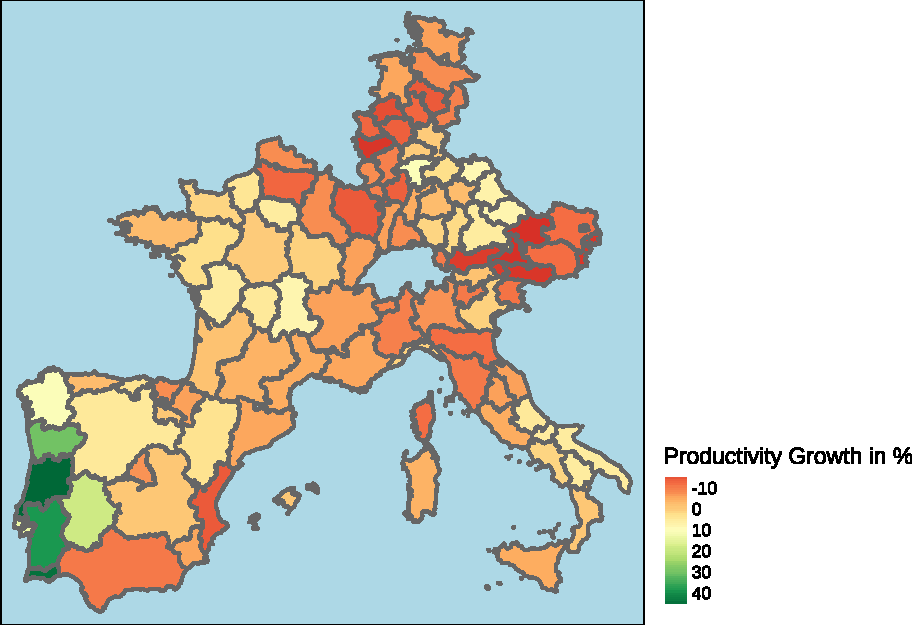
\includegraphics{02_assignmnet_files/figure-latex/unnamed-chunk-2-1.pdf}

\hypertarget{generate-three-different-spatial-weights-matrixes-using-i-a-distance-threshold-ii-smooth-distance-decay-and-iii-a-contiguity-based-measure.}{%
\subsection{Generate three different spatial weights matrixes using (i)
a distance threshold, (ii) smooth distance-decay, and iii) a
contiguity-based
measure.}\label{generate-three-different-spatial-weights-matrixes-using-i-a-distance-threshold-ii-smooth-distance-decay-and-iii-a-contiguity-based-measure.}}

\hypertarget{i-distance-threshold}{%
\subsubsection{(i) Distance Threshold}\label{i-distance-threshold}}

First, we create a binary distance threshold spatial weights matrix
based. Any region is being assigned a `1' with respect to another
region, if it is less than 3 km away. We have chosen this threshold so
that every region has a neighbor. We use the nb2mat function from the
`spdep' package. We row-normalize the matrix.

\begin{Shaded}
\begin{Highlighting}[]
\NormalTok{coords }\OtherTok{\textless{}{-}} \FunctionTok{st\_coordinates}\NormalTok{(}\FunctionTok{st\_centroid}\NormalTok{(EU27))}

\CommentTok{\#checking the maximum distance as to include all observations which have a matrix   }
\NormalTok{nb1 }\OtherTok{\textless{}{-}} \FunctionTok{knn2nb}\NormalTok{(}\FunctionTok{knearneigh}\NormalTok{(coords, }\AttributeTok{k =} \DecValTok{1}\NormalTok{))}

\NormalTok{dist1 }\OtherTok{\textless{}{-}} \FunctionTok{nbdists}\NormalTok{(nb1, coords)}

\NormalTok{distw }\OtherTok{\textless{}{-}} \FunctionTok{dnearneigh}\NormalTok{(coords, }\DecValTok{0}\NormalTok{, }\DecValTok{3}\NormalTok{)}

\CommentTok{\#creating matrix based on distance threshold up to 3 kilometers}
\NormalTok{dist\_w\_matrix }\OtherTok{\textless{}{-}} \FunctionTok{nb2mat}\NormalTok{(distw, }\AttributeTok{style=}\StringTok{"W"}\NormalTok{, }\AttributeTok{zero.policy=}\ConstantTok{TRUE}\NormalTok{)}
\end{Highlighting}
\end{Shaded}

\hypertarget{ii-smooth-distance-decay}{%
\subsubsection{(ii) Smooth-Distance
Decay}\label{ii-smooth-distance-decay}}

Next, we create a spatial weights matrix based on a smooth
distance-decay. We use the following simple distance decay function
\(w_{i, j} = 1/d_{i,j}^{\lambda}\), where d denotes the distance between
observation i and j, and \(\lambda\) is the distance decay parameter. By
ease of convention we set \(\lambda = 0\). We calculate the weights for
each neighboring region based on the k=20 nearest neighbors. We do
\textit{not} row-normalize the matrix.

\begin{Shaded}
\begin{Highlighting}[]
\NormalTok{k1 }\OtherTok{\textless{}{-}} \FunctionTok{knearneigh}\NormalTok{(coords, }\AttributeTok{k=}\DecValTok{20}\NormalTok{)}
\NormalTok{k2 }\OtherTok{\textless{}{-}} \FunctionTok{knn2nb}\NormalTok{(k1)}

\NormalTok{dists }\OtherTok{\textless{}{-}} \FunctionTok{nbdists}\NormalTok{(k2, coords)}

\NormalTok{ids }\OtherTok{\textless{}{-}} \FunctionTok{lapply}\NormalTok{(dists, }\ControlFlowTok{function}\NormalTok{(d)\{}\DecValTok{1}\SpecialCharTok{/}\NormalTok{d\})}

\NormalTok{decay\_weights\_matrix\_list }\OtherTok{\textless{}{-}} \FunctionTok{nb2listw}\NormalTok{(k2, }\AttributeTok{glist =}\NormalTok{ ids, }\AttributeTok{style =} \StringTok{"B"}\NormalTok{, }\AttributeTok{zero.policy =} \ConstantTok{TRUE}\NormalTok{)}

\NormalTok{decay\_weights\_matrix }\OtherTok{\textless{}{-}} \FunctionTok{listw2mat}\NormalTok{(decay\_weights\_matrix\_list)}
\end{Highlighting}
\end{Shaded}

\hypertarget{iii-contiguity-based-measure}{%
\subsubsection{(iii) Contiguity-based
measure}\label{iii-contiguity-based-measure}}

Finally, we calculate a contiguity based measure, which we row normalize
as well.

\begin{Shaded}
\begin{Highlighting}[]
\CommentTok{\# Create a contiguity{-}based spatial weights matrix}
\NormalTok{queen\_weights }\OtherTok{\textless{}{-}} \FunctionTok{poly2nb}\NormalTok{(EU27, }\AttributeTok{queen =} \ConstantTok{TRUE}\NormalTok{)}

\NormalTok{contig\_w\_matrix }\OtherTok{\textless{}{-}} \FunctionTok{nb2mat}\NormalTok{(queen\_weights, }\AttributeTok{style=}\StringTok{"W"}\NormalTok{, }\AttributeTok{zero.policy=}\ConstantTok{TRUE}\NormalTok{)}
\end{Highlighting}
\end{Shaded}

\hypertarget{compare-the-matrices-use-your-knowledge-of-graph-theory-and-linear-algebra}{%
\subsection{Compare the matrices; use your knowledge of graph theory and
linear
algebra}\label{compare-the-matrices-use-your-knowledge-of-graph-theory-and-linear-algebra}}

We can gain deeper insights into these spatial weights matrices as well
as the networks they represent by comparing key measures of the graphs
that are derived from them.

\begin{table}

\caption{\label{tab:unnamed-chunk-7}Summary of Distance Threshold Graph}
\centering
\begin{tabular}[t]{l|l}
\hline
Property & Value\\
\hline
Number of vertices & 103\\
\hline
Number of edges & 514\\
\hline
Average path length & 0.6750662\\
\hline
Graph density & 0.09784885\\
\hline
Average degree & 9.980583\\
\hline
Max Eigenvector Centrality & 1\\
\hline
Min Eigenvector Centrality & 0.008694479\\
\hline
Average Eigenvector Centrality & 0.1497447\\
\hline
Most Central Unit (Vertex ID) & 49\\
\hline
\end{tabular}
\end{table}

\begin{table}

\caption{\label{tab:unnamed-chunk-7}Summary of Smooth Distance-Decay Matrix}
\centering
\begin{tabular}[t]{l|l}
\hline
Property & Value\\
\hline
Number of vertices & 103\\
\hline
Number of edges & 1266\\
\hline
Average path length & 0.49328\\
\hline
Graph density & 0.2410051\\
\hline
Average degree & 24.58252\\
\hline
Max Eigenvector Centrality & 1\\
\hline
Min Eigenvector Centrality & 0.001002582\\
\hline
Average Eigenvector Centrality & 0.2836761\\
\hline
Most Central Unit (Vertex ID) & 23\\
\hline
\end{tabular}
\end{table}

\begin{table}

\caption{\label{tab:unnamed-chunk-7}Summary of Contiguity-Based Graph}
\centering
\begin{tabular}[t]{l|l}
\hline
Property & Value\\
\hline
Number of vertices & 103\\
\hline
Number of edges & 222\\
\hline
Average path length & 1.288804\\
\hline
Graph density & 0.04226156\\
\hline
Average degree & 4.31068\\
\hline
Max Eigenvector Centrality & 1\\
\hline
Min Eigenvector Centrality & 0\\
\hline
Average Eigenvector Centrality & 0.08975192\\
\hline
Most Central Unit (Vertex ID) & 48\\
\hline
\end{tabular}
\end{table}

We compare the matrices based on a set of characteristics. We compare
the row-normalized matrices for the queen contiguity and distance
threshold matrix. Note that normalization procedure does not preserve
the structure of the network.

\textbf{Number of edges}

The Smooth Distance-Decay Graph has the most edges (1266). The Distance
Threshold Graph has fewer edges (514) than the Smooth Distance-Decay
Graph, implying stricter criteria for edge creation based on a fixed
distance threshold. The Contiguity-Based Graph has the fewest edges
(222), since only directly contiguous or neighboring entities are
connected, leading to a more sparse graph structure.

\textbf{Average path length}

The Contiguity-Based Graph has the highest average path length (1.2888),
reflecting the sparse connectivity where nodes are less directly
connected. The Distance Threshold Graph has a medium average path length
(0.6751). The Smooth Distance-Decay Graph has the lowest average path
length (0.4933), indicative of a denser network where nodes are more
directly accessible to one another.

\textbf{Graph density}

Consistent with the number of edges, the Smooth Distance-Decay Graph is
the densest (0.2410), followed by the Distance Threshold Graph (0.0978),
with the Contiguity-Based Graph being the least dense (0.0423).

\textbf{Average degree}

Again, the Smooth Distance-Decay Graph shows the highest average degree
(24.5825), the Distance Threshold Graph shows a medium degree (9.9806),
and the Contiguity-Based Graph has the lowest (4.3107).

\textbf{Minimum Eigenvector Centrality}

The Contiguity-Based Graph shows the most significant variation in
centrality (minimum near zero), reflecting a few very poorly connected
nodes, or nodes that only connect to other low-influence nodes. The
Smooth Distance-Decay Graph and the Distance Threshold Graph have higher
minimum values, indicating a more uniform distribution of node
influence.

\textbf{Average Eigenvector Centrality}

Higher on average in the Smooth Distance-Decay Graph (0.2837),
suggesting that, on average, nodes are better positioned or more
influential within the network. It's lowest in the Contiguity-Based
Graph (0.0898), consistent with its sparse and uneven connectivity.

Looking at the most central unit through eigenvector centrality shows
that different nodes are identified as most central in each graph,
reflecting the impact of the underlying connection logic on the
perceived importance or centrality of nodes.

\hypertarget{plot-the-matrix}{%
\subsection{Plot the matrix}\label{plot-the-matrix}}

We now plot the three spatial weight matrices. We see that the distance
decay weight matrix is symmetric. The distance decay matrix is

\begin{center}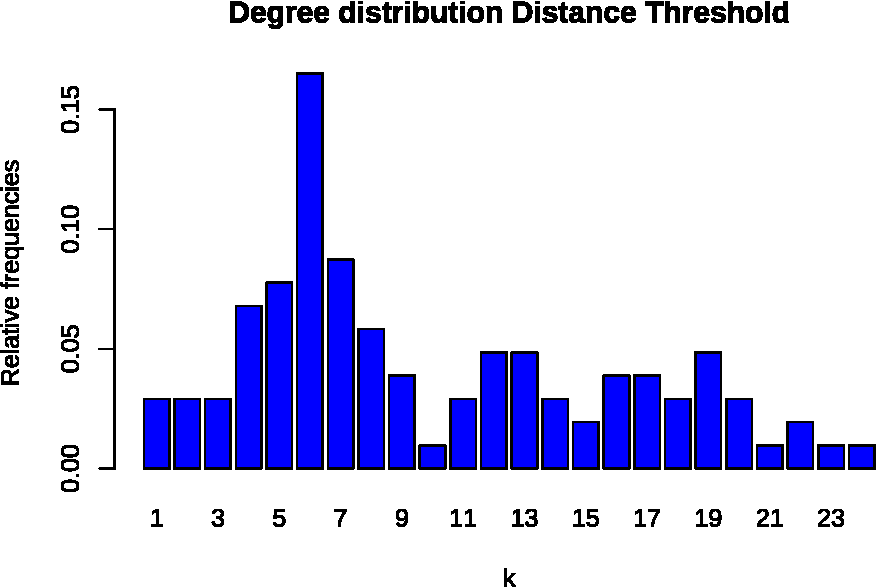
\includegraphics{02_assignmnet_files/figure-latex/unnamed-chunk-8-1} \end{center}

\begin{center}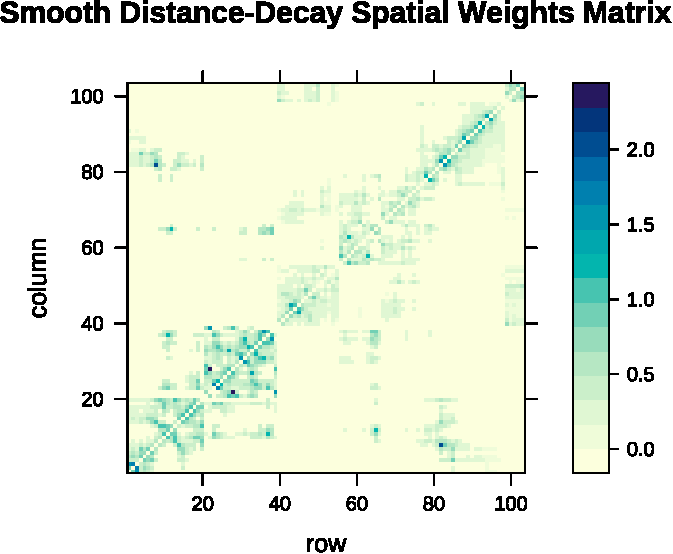
\includegraphics{02_assignmnet_files/figure-latex/unnamed-chunk-8-2} \end{center}

\begin{center}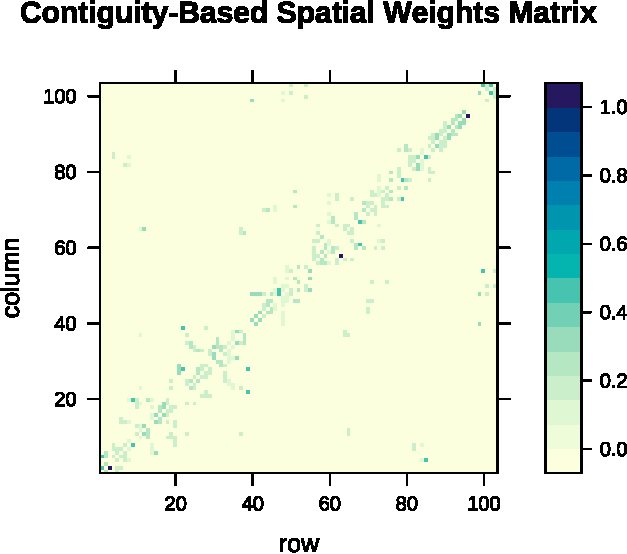
\includegraphics{02_assignmnet_files/figure-latex/unnamed-chunk-8-3} \end{center}

\hypertarget{try-to-visualize-the-network-they-represent}{%
\subsection{Try to visualize the network they
represent}\label{try-to-visualize-the-network-they-represent}}

Let us first visualize the distance based spatial matrix. The first plot
shows the map of Europe and the blue lines indicate the connections. The
map shows the connectivity in Europe based on the distance threshold.

The second map visualizes the network based on the distance decay
matrix. However, the edges do not display the intensity of connections,
but just the connectivity to neighboring regions.

The last map displays the queen contiguity based measure. The islands in
the middle sea are not being counted as neighbors. This should caution
the use of this network, as it seems implausible that Siciliy for
example is not connected to the mainland Italian provinces.

\begin{center}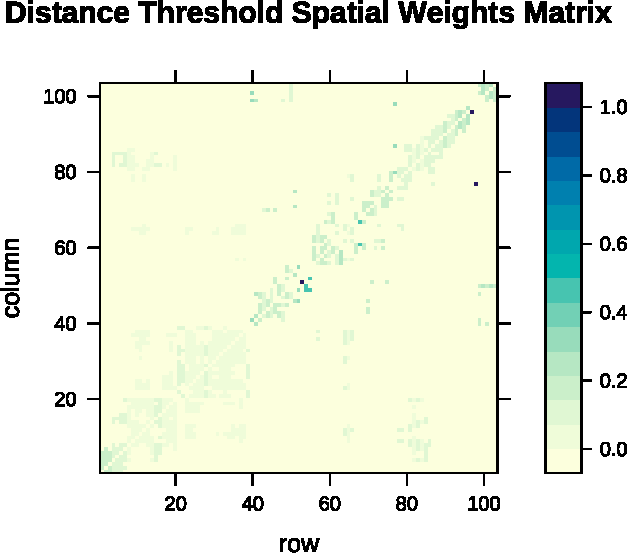
\includegraphics{02_assignmnet_files/figure-latex/unnamed-chunk-9-1} \end{center}

\hypertarget{compute-a-suitable-measure-of-spatial-autocorrelation-for-productivity-growth-using-these-matrices.-point-out-differences-if-there-are-any.}{%
\subsection{Compute a suitable measure of spatial autocorrelation for
productivity growth using these matrices. Point out differences, if
there are
any.}\label{compute-a-suitable-measure-of-spatial-autocorrelation-for-productivity-growth-using-these-matrices.-point-out-differences-if-there-are-any.}}

We calculate Global Moran's I as a measure of spatial autocorrelation
for all three spatial weight matrices. All three matrices display the
strong positive spatial autocorrelation between 0.62 - 0.54, which are
all highly statistically significant with p-values \textless{} 0.01.
Thus there is strong evidence for the presence of sizeable levels of
spatial autocorrelation. This result is robust to the choice of the
spatial weights matrix.

\begin{table}
\centering
\resizebox{\linewidth}{!}{
\begin{tabular}{>{}l|rrr>{}r}
\toprule
Test & Moran\_I & Expectation & Variance & p\_value\\
\midrule
\textbf{\cellcolor{gray!6}{Distance Threshold}} & \cellcolor{gray!6}{0.5938} & \cellcolor{gray!6}{-0.0098} & \cellcolor{gray!6}{0.0026} & \textcolor{red}{\cellcolor{gray!6}{0}}\\
\textbf{Smooth Distance-Decay} & 0.2925 & -0.0098 & 0.0010 & \textcolor{red}{0}\\
\textbf{\cellcolor{gray!6}{Contiguity-Based}} & \cellcolor{gray!6}{0.5380} & \cellcolor{gray!6}{-0.0102} & \cellcolor{gray!6}{0.0045} & \textcolor{red}{\cellcolor{gray!6}{0}}\\
\bottomrule
\end{tabular}}
\end{table}

\hypertarget{estimate-a-linear-regression-model-using-ols.}{%
\subsection{Estimate a linear regression model using
OLS.}\label{estimate-a-linear-regression-model-using-ols.}}

We estimate the specified model and obtain the following output.

\begin{table}[!htbp] \centering 
  \caption{} 
  \label{} 
\begin{tabular}{@{\extracolsep{5pt}}lc} 
\\[-1.8ex]\hline 
\hline \\[-1.8ex] 
 & \multicolumn{1}{c}{\textit{Dependent variable:}} \\ 
\cline{2-2} 
\\[-1.8ex] & prod\_growth \\ 
\hline \\[-1.8ex] 
 pr80b & $-$0.253$^{***}$ \\ 
  & (0.025) \\ 
  & \\ 
 lninv1b & 0.032$^{***}$ \\ 
  & (0.008) \\ 
  & \\ 
 lndens.empb & 0.007 \\ 
  & (0.009) \\ 
  & \\ 
 Constant & 0.314$^{***}$ \\ 
  & (0.061) \\ 
  & \\ 
\hline \\[-1.8ex] 
Observations & 103 \\ 
R$^{2}$ & 0.528 \\ 
Adjusted R$^{2}$ & 0.514 \\ 
Residual Std. Error & 0.080 (df = 99) \\ 
F Statistic & 36.983$^{***}$ (df = 3; 99) \\ 
\hline 
\hline \\[-1.8ex] 
\textit{Note:}  & \multicolumn{1}{r}{$^{*}$p$<$0.1; $^{**}$p$<$0.05; $^{***}$p$<$0.01} \\ 
\end{tabular} 
\end{table}

We observe strong evidence for spatial autocorrelation. This holds for
all spatial weights matrices used. The different weighting schemes
highlight differnt countries. Thus the neglect fo this spatial dimension
might give rise to bias in the OLS estimated coefficients.

\begin{center}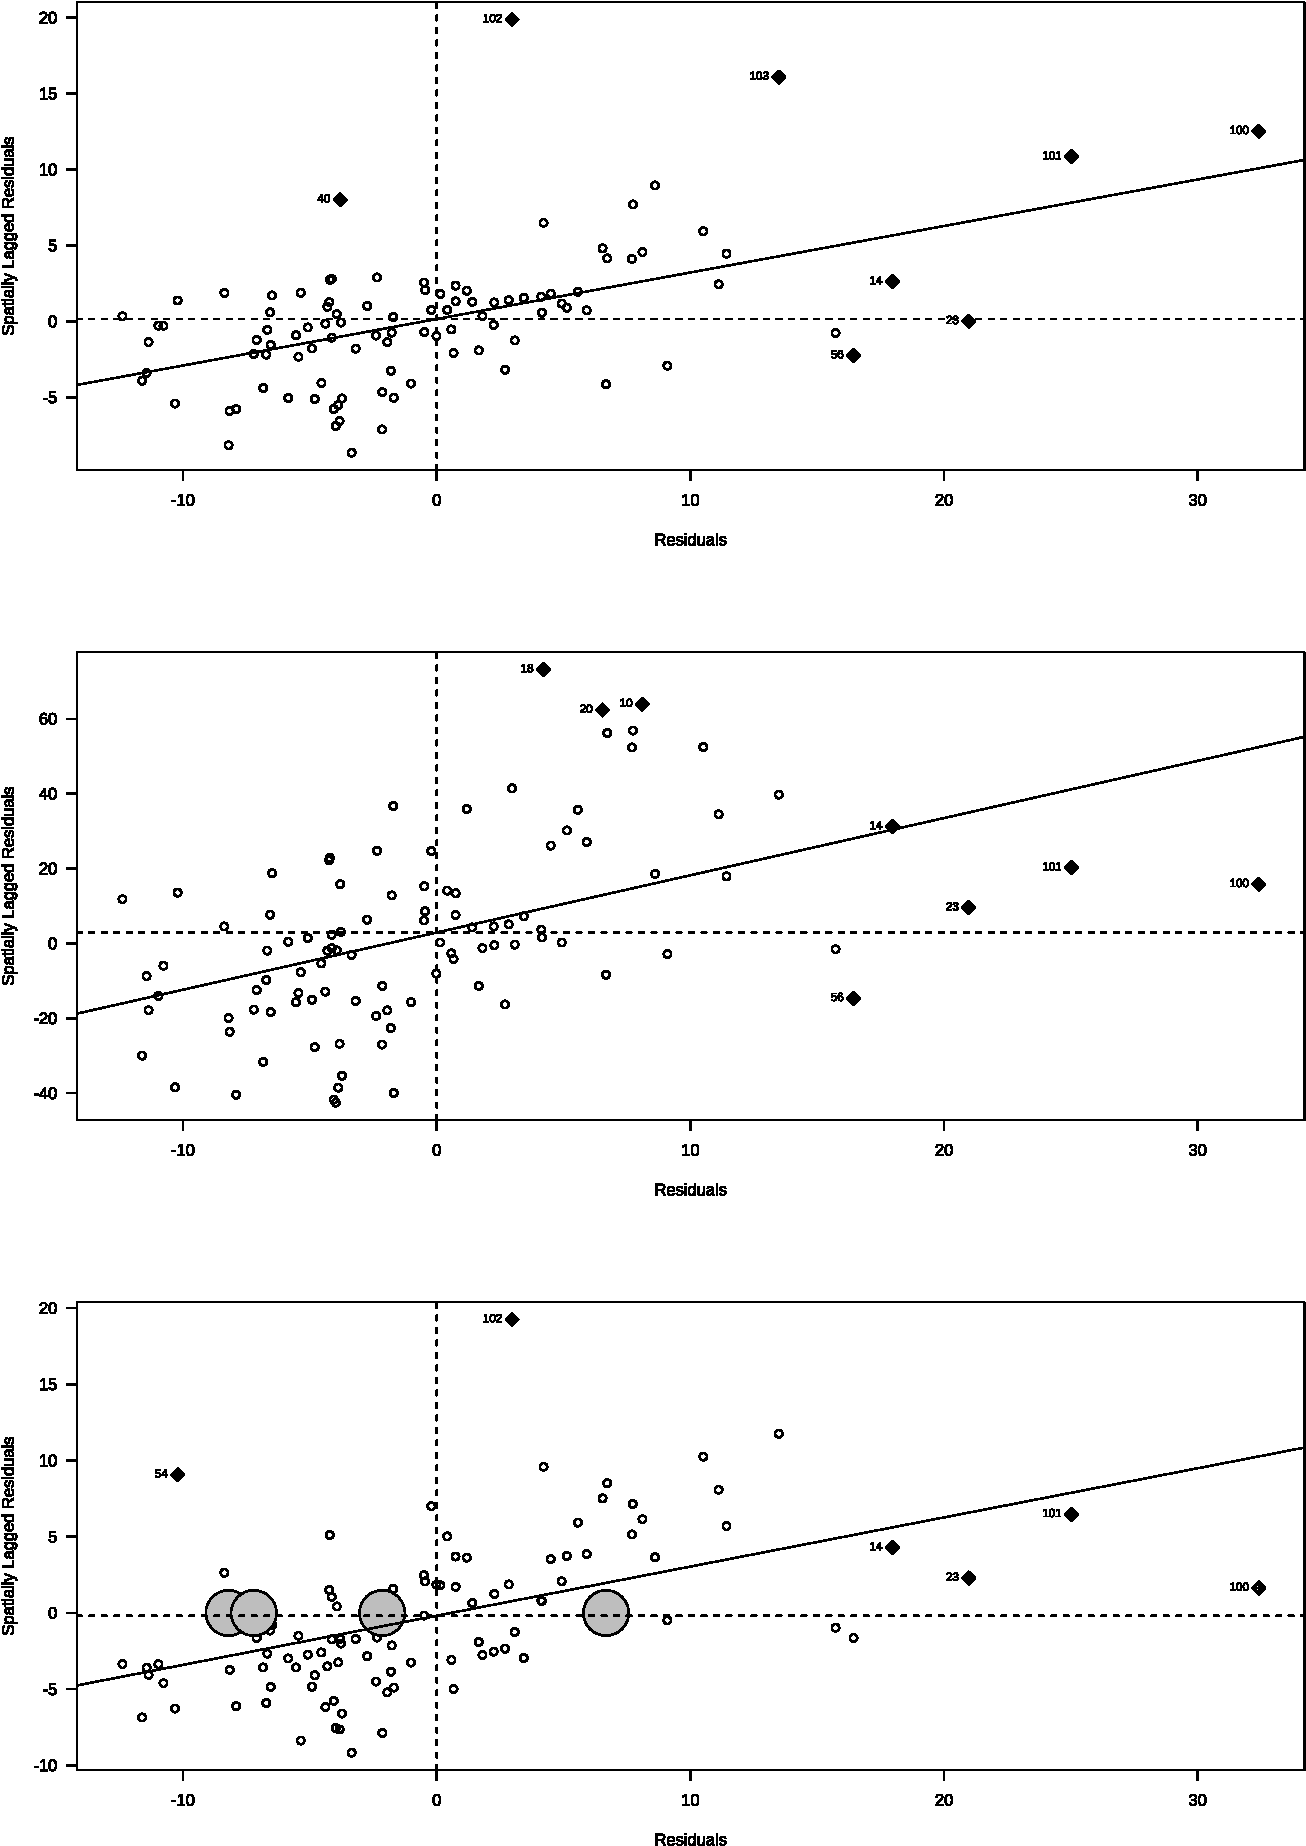
\includegraphics{02_assignmnet_files/figure-latex/unnamed-chunk-11-1} \end{center}

\hypertarget{exercise-b}{%
\section{Exercise B}\label{exercise-b}}

\hypertarget{creating-maps}{%
\subsection{Creating maps}\label{creating-maps}}

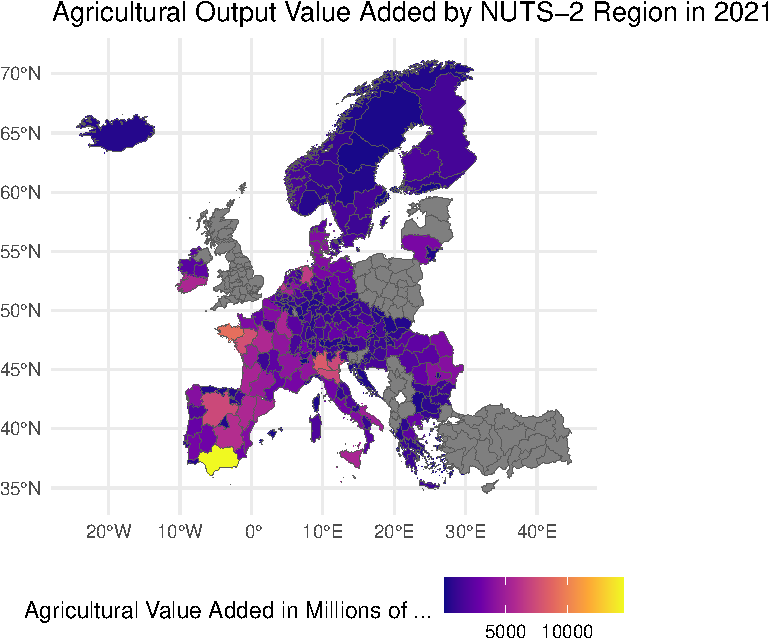
\includegraphics{02_assignmnet_files/figure-latex/unnamed-chunk-13-1.pdf}

We now replicate table 2

\begin{Shaded}
\begin{Highlighting}[]
\NormalTok{list\_2 }\OtherTok{\textless{}{-}}\NormalTok{ dat2 }\SpecialCharTok{\%\textgreater{}\%}
  \FunctionTok{select}\NormalTok{(COUNTRY, geometry, NAME\_1, NAME\_2) }\SpecialCharTok{\%\textgreater{}\%}
  \FunctionTok{mutate}\NormalTok{(}\AttributeTok{country =} \FunctionTok{ifelse}\NormalTok{(COUNTRY }\SpecialCharTok{==} \StringTok{"Brazil"}\NormalTok{, }\StringTok{"BRA"}\NormalTok{, COUNTRY)) }\SpecialCharTok{\%\textgreater{}\%}
  \FunctionTok{rename}\NormalTok{(}\StringTok{"muni"} \OtherTok{=} \StringTok{"NAME\_2"}\NormalTok{) }\SpecialCharTok{\%\textgreater{}\%}
  \FunctionTok{mutate}\NormalTok{(}\AttributeTok{state =} \FunctionTok{ifelse}\NormalTok{(NAME\_1 }\SpecialCharTok{==} \StringTok{"Rio Grande do Sul"}\NormalTok{, }\StringTok{"RS"}\NormalTok{, NAME\_1)) }

\NormalTok{literacy\_Arg\_Bra\_Par\_2 }\OtherTok{\textless{}{-}}\NormalTok{ literacy\_Arg\_Bra\_Par }\SpecialCharTok{\%\textgreater{}\%}
  \FunctionTok{left\_join}\NormalTok{(list\_2, }\AttributeTok{by =} \FunctionTok{c}\NormalTok{(}\StringTok{"muni"}\NormalTok{,  }\StringTok{"state"}\NormalTok{, }\StringTok{"country"}\NormalTok{))}

\NormalTok{mod1 }\OtherTok{\textless{}{-}} \FunctionTok{lm}\NormalTok{(illiteracy }\SpecialCharTok{\textasciitilde{}}\NormalTok{ (lati) }\SpecialCharTok{+}\NormalTok{ (longi) }\SpecialCharTok{+}\NormalTok{ distmiss }\SpecialCharTok{+}\NormalTok{ state, }\AttributeTok{data =}\NormalTok{ literacy\_Arg\_Bra\_Par\_2)}

\NormalTok{mod2 }\OtherTok{\textless{}{-}} \FunctionTok{lm}\NormalTok{(illiteracy }\SpecialCharTok{\textasciitilde{}}\NormalTok{ (lati) }\SpecialCharTok{+}\NormalTok{ (longi) }\SpecialCharTok{+}\NormalTok{ distmiss }\SpecialCharTok{+}\NormalTok{ state }\SpecialCharTok{+}\NormalTok{ coast }\SpecialCharTok{+}\NormalTok{ river }\SpecialCharTok{+}\NormalTok{ slope }\SpecialCharTok{+}\NormalTok{ rugg }\SpecialCharTok{+}\NormalTok{ alti }\SpecialCharTok{+}\NormalTok{ tempe }\SpecialCharTok{+}\NormalTok{ preci }\SpecialCharTok{+}\NormalTok{ area, }\AttributeTok{data =}\NormalTok{ literacy\_Arg\_Bra\_Par\_2)}


\NormalTok{bra }\OtherTok{\textless{}{-}}\NormalTok{ literacy\_Arg\_Bra\_Par\_2 }\SpecialCharTok{\%\textgreater{}\%} 
             \FunctionTok{filter}\NormalTok{(country }\SpecialCharTok{==} \StringTok{"BRA"}\NormalTok{)}

\NormalTok{mod3 }\OtherTok{\textless{}{-}} \FunctionTok{lm}\NormalTok{(illiteracy }\SpecialCharTok{\textasciitilde{}}\NormalTok{ (lati) }\SpecialCharTok{+}\NormalTok{ (longi) }\SpecialCharTok{+}\NormalTok{ distmiss }\SpecialCharTok{+}\NormalTok{ mesorregi, }\AttributeTok{data =}\NormalTok{ bra)}

\NormalTok{mod4 }\OtherTok{\textless{}{-}} \FunctionTok{lm}\NormalTok{(illiteracy }\SpecialCharTok{\textasciitilde{}}\NormalTok{ (lati) }\SpecialCharTok{+}\NormalTok{ (longi) }\SpecialCharTok{+}\NormalTok{ distmiss }\SpecialCharTok{+}\NormalTok{ mesorregi }\SpecialCharTok{+}\NormalTok{ coast }\SpecialCharTok{+}\NormalTok{ river }\SpecialCharTok{+}\NormalTok{ slope }\SpecialCharTok{+}\NormalTok{ rugg }\SpecialCharTok{+}\NormalTok{ alti }\SpecialCharTok{+}\NormalTok{ tempe }\SpecialCharTok{+}\NormalTok{ preci }\SpecialCharTok{+}\NormalTok{ area, }\AttributeTok{data =}\NormalTok{ bra)}


\NormalTok{arg }\OtherTok{\textless{}{-}}\NormalTok{ literacy\_Arg\_Bra\_Par\_2 }\SpecialCharTok{\%\textgreater{}\%} 
             \FunctionTok{filter}\NormalTok{(country }\SpecialCharTok{==} \StringTok{"Argentina"}\NormalTok{)}

\NormalTok{mod5 }\OtherTok{\textless{}{-}} \FunctionTok{lm}\NormalTok{(illiteracy }\SpecialCharTok{\textasciitilde{}}\NormalTok{ (lati) }\SpecialCharTok{+}\NormalTok{ (longi) }\SpecialCharTok{+}\NormalTok{ distmiss, }\AttributeTok{data =}\NormalTok{ arg)}

\NormalTok{mod6 }\OtherTok{\textless{}{-}} \FunctionTok{lm}\NormalTok{(illiteracy }\SpecialCharTok{\textasciitilde{}}\NormalTok{ (lati) }\SpecialCharTok{+}\NormalTok{ (longi) }\SpecialCharTok{+}\NormalTok{ distmiss }\SpecialCharTok{+}\NormalTok{ coast }\SpecialCharTok{+}\NormalTok{ river }\SpecialCharTok{+}\NormalTok{ slope }\SpecialCharTok{+}\NormalTok{ rugg }\SpecialCharTok{+}\NormalTok{ alti }\SpecialCharTok{+}\NormalTok{ tempe }\SpecialCharTok{+}\NormalTok{ preci }\SpecialCharTok{+}\NormalTok{ area, }\AttributeTok{data =}\NormalTok{ arg)}


\NormalTok{par }\OtherTok{\textless{}{-}}\NormalTok{ literacy\_Arg\_Bra\_Par\_2 }\SpecialCharTok{\%\textgreater{}\%} 
             \FunctionTok{filter}\NormalTok{(country }\SpecialCharTok{==} \StringTok{"Paraguay"}\NormalTok{)}

\NormalTok{mod7 }\OtherTok{\textless{}{-}} \FunctionTok{lm}\NormalTok{(illiteracy }\SpecialCharTok{\textasciitilde{}}\NormalTok{ (lati) }\SpecialCharTok{+}\NormalTok{ (longi) }\SpecialCharTok{+}\NormalTok{ distmiss }\SpecialCharTok{+}\NormalTok{ state, }\AttributeTok{data =}\NormalTok{ par)}

\NormalTok{mod8 }\OtherTok{\textless{}{-}} \FunctionTok{lm}\NormalTok{(illiteracy }\SpecialCharTok{\textasciitilde{}}\NormalTok{ (lati) }\SpecialCharTok{+}\NormalTok{ (longi) }\SpecialCharTok{+}\NormalTok{ distmiss }\SpecialCharTok{+}\NormalTok{ state }\SpecialCharTok{+}\NormalTok{ coast }\SpecialCharTok{+}\NormalTok{ river }\SpecialCharTok{+}\NormalTok{ slope }\SpecialCharTok{+}\NormalTok{ rugg }\SpecialCharTok{+}\NormalTok{ alti }\SpecialCharTok{+}\NormalTok{ tempe }\SpecialCharTok{+}\NormalTok{ preci }\SpecialCharTok{+}\NormalTok{ area, }\AttributeTok{data =}\NormalTok{ par)}

\FunctionTok{stargazer}\NormalTok{(mod1, mod2, mod3, mod4, mod5, mod6, mod7, mod8)}
\end{Highlighting}
\end{Shaded}

\begin{verbatim}
## 
## % Table created by stargazer v.5.2.3 by Marek Hlavac, Social Policy Institute. E-mail: marek.hlavac at gmail.com
## % Date and time: Sun, Apr 14, 2024 - 19:55:26
## \begin{table}[!htbp] \centering 
##   \caption{} 
##   \label{} 
## \begin{tabular}{@{\extracolsep{5pt}}lcccccccc} 
## \\[-1.8ex]\hline 
## \hline \\[-1.8ex] 
##  & \multicolumn{8}{c}{\textit{Dependent variable:}} \\ 
## \cline{2-9} 
## \\[-1.8ex] & \multicolumn{8}{c}{illiteracy} \\ 
## \\[-1.8ex] & (1) & (2) & (3) & (4) & (5) & (6) & (7) & (8)\\ 
## \hline \\[-1.8ex] 
##  lati & 0.556$^{**}$ & 0.072 & 0.359 & 3.206$^{**}$ & 0.043 & $-$6.724$^{**}$ & 3.540$^{**}$ & $-$7.429 \\ 
##   & (0.251) & (0.782) & (0.403) & (1.473) & (0.643) & (2.599) & (1.622) & (4.381) \\ 
##   & & & & & & & & \\ 
##  longi & $-$1.108$^{***}$ & $-$1.007 & $-$1.716$^{***}$ & $-$5.054$^{***}$ & 0.054 & 6.704$^{***}$ & 0.298 & 20.866$^{***}$ \\ 
##   & (0.269) & (0.687) & (0.369) & (1.521) & (0.496) & (1.934) & (1.017) & (6.364) \\ 
##   & & & & & & & & \\ 
##  distmiss & 0.011$^{***}$ & 0.011$^{**}$ & 0.020$^{***}$ & 0.031$^{***}$ & 0.013 & 0.055$^{***}$ & $-$0.035 & $-$0.071$^{**}$ \\ 
##   & (0.004) & (0.005) & (0.006) & (0.008) & (0.008) & (0.019) & (0.023) & (0.029) \\ 
##   & & & & & & & & \\ 
##  stateItapúa & 2.154 & 3.619$^{**}$ &  &  &  &  &  &  \\ 
##   & (1.350) & (1.693) &  &  &  &  &  &  \\ 
##   & & & & & & & & \\ 
##  stateMisiones & 1.017 & 1.297 &  &  &  &  & 0.200 & $-$2.053 \\ 
##   & (1.572) & (1.865) &  &  &  &  & (1.481) & (1.661) \\ 
##   & & & & & & & & \\ 
##  stateMisiones1 & 2.061 & 3.733$^{**}$ &  &  &  &  &  &  \\ 
##   & (1.565) & (1.881) &  &  &  &  &  &  \\ 
##   & & & & & & & & \\ 
##  stateRS & 5.341$^{***}$ & 6.027$^{***}$ &  &  &  &  &  &  \\ 
##   & (1.521) & (1.798) &  &  &  &  &  &  \\ 
##   & & & & & & & & \\ 
##  coast &  & 0.209 &  & $-$3.864$^{**}$ &  & $-$0.764 &  & 21.631$^{***}$ \\ 
##   &  & (0.989) &  & (1.848) &  & (2.857) &  & (7.366) \\ 
##   & & & & & & & & \\ 
##  river &  & 1.465$^{**}$ &  & 1.645$^{**}$ &  & 10.574$^{***}$ &  & $-$4.913 \\ 
##   &  & (0.741) &  & (0.802) &  & (2.672) &  & (4.569) \\ 
##   & & & & & & & & \\ 
##  slope &  & $-$0.00001 &  & 0.00002 &  & $-$0.053$^{*}$ &  & $-$0.071$^{***}$ \\ 
##   &  & (0.0002) &  & (0.0002) &  & (0.028) &  & (0.021) \\ 
##   & & & & & & & & \\ 
##  rugg &  & $-$0.00000 &  & $-$0.00000 &  & 0.001$^{*}$ &  & 0.002$^{***}$ \\ 
##   &  & (0.00000) &  & (0.00000) &  & (0.001) &  & (0.001) \\ 
##   & & & & & & & & \\ 
##  alti &  & 0.006 &  & 0.005 &  & 0.062$^{***}$ &  & 0.038$^{**}$ \\ 
##   &  & (0.004) &  & (0.005) &  & (0.011) &  & (0.014) \\ 
##   & & & & & & & & \\ 
##  tempe &  & 0.058 &  & 0.057 &  & 0.915$^{***}$ &  & 0.842$^{***}$ \\ 
##   &  & (0.079) &  & (0.099) &  & (0.208) &  & (0.204) \\ 
##   & & & & & & & & \\ 
##  preci &  & $-$0.003 &  & $-$0.002 &  & $-$0.019$^{**}$ &  & $-$0.012$^{**}$ \\ 
##   &  & (0.002) &  & (0.002) &  & (0.007) &  & (0.005) \\ 
##   & & & & & & & & \\ 
##  area &  & 0.0001 &  & $-$0.0004 &  & $-$0.0003 &  & 0.002$^{***}$ \\ 
##   &  & (0.0002) &  & (0.0003) &  & (0.0002) &  & (0.001) \\ 
##   & & & & & & & & \\ 
##  mesorregi &  &  & $-$0.418$^{*}$ & $-$0.216 &  &  &  &  \\ 
##   &  &  & (0.216) & (0.261) &  &  &  &  \\ 
##   & & & & & & & & \\ 
##  Constant & $-$40.669$^{***}$ & $-$59.567 & 1,724.668$^{*}$ & 755.296 & 11.554 & 31.195 & 121.370$^{*}$ & 685.427$^{***}$ \\ 
##   & (13.191) & (36.199) & (919.888) & (1,111.741) & (20.002) & (72.708) & (60.387) & (208.813) \\ 
##   & & & & & & & & \\ 
## \hline \\[-1.8ex] 
## Observations & 549 & 548 & 467 & 467 & 42 & 42 & 40 & 39 \\ 
## R$^{2}$ & 0.042 & 0.073 & 0.056 & 0.095 & 0.099 & 0.695 & 0.145 & 0.652 \\ 
## Adjusted R$^{2}$ & 0.029 & 0.047 & 0.048 & 0.071 & 0.028 & 0.583 & 0.047 & 0.491 \\ 
## Residual Std. Error & 3.948 (df = 541) & 3.916 (df = 532) & 4.101 (df = 462) & 4.050 (df = 454) & 2.997 (df = 38) & 1.962 (df = 30) & 2.048 (df = 35) & 1.513 (df = 26) \\ 
## F Statistic & 3.370$^{***}$ (df = 7; 541) & 2.793$^{***}$ (df = 15; 532) & 6.880$^{***}$ (df = 4; 462) & 3.976$^{***}$ (df = 12; 454) & 1.396 (df = 3; 38) & 6.218$^{***}$ (df = 11; 30) & 1.482 (df = 4; 35) & 4.058$^{***}$ (df = 12; 26) \\ 
## \hline 
## \hline \\[-1.8ex] 
## \textit{Note:}  & \multicolumn{8}{r}{$^{*}$p$<$0.1; $^{**}$p$<$0.05; $^{***}$p$<$0.01} \\ 
## \end{tabular} 
## \end{table}
\end{verbatim}

\begin{table}[!htbp] \centering 
  \caption{} 
  \label{} 
\begin{tabular}{@{\extracolsep{5pt}}lcccccccc} 
\\[-1.8ex]\hline 
\hline \\[-1.8ex] 
 & \multicolumn{8}{c}{\textit{Dependent variable:}} \\ 
\cline{2-9} 
\\[-1.8ex] & \multicolumn{8}{c}{illiteracy} \\ 
\\[-1.8ex] & (1) & (2) & (3) & (4) & (5) & (6) & (7) & (8)\\ 
\hline \\[-1.8ex] 
 lati & 0.556$^{**}$ & 0.072 & 0.359 & 3.206$^{**}$ & 0.043 & $-$6.724$^{**}$ & 3.540$^{**}$ & $-$7.429 \\ 
  & (0.251) & (0.782) & (0.403) & (1.473) & (0.643) & (2.599) & (1.622) & (4.381) \\ 
  & & & & & & & & \\ 
 longi & $-$1.108$^{***}$ & $-$1.007 & $-$1.716$^{***}$ & $-$5.054$^{***}$ & 0.054 & 6.704$^{***}$ & 0.298 & 20.866$^{***}$ \\ 
  & (0.269) & (0.687) & (0.369) & (1.521) & (0.496) & (1.934) & (1.017) & (6.364) \\ 
  & & & & & & & & \\ 
 distmiss & 0.011$^{***}$ & 0.011$^{**}$ & 0.020$^{***}$ & 0.031$^{***}$ & 0.013 & 0.055$^{***}$ & $-$0.035 & $-$0.071$^{**}$ \\ 
  & (0.004) & (0.005) & (0.006) & (0.008) & (0.008) & (0.019) & (0.023) & (0.029) \\ 
  & & & & & & & & \\ 
 stateItapúa & 2.154 & 3.619$^{**}$ &  &  &  &  &  &  \\ 
  & (1.350) & (1.693) &  &  &  &  &  &  \\ 
  & & & & & & & & \\ 
 stateMisiones & 1.017 & 1.297 &  &  &  &  & 0.200 & $-$2.053 \\ 
  & (1.572) & (1.865) &  &  &  &  & (1.481) & (1.661) \\ 
  & & & & & & & & \\ 
 stateMisiones1 & 2.061 & 3.733$^{**}$ &  &  &  &  &  &  \\ 
  & (1.565) & (1.881) &  &  &  &  &  &  \\ 
  & & & & & & & & \\ 
 stateRS & 5.341$^{***}$ & 6.027$^{***}$ &  &  &  &  &  &  \\ 
  & (1.521) & (1.798) &  &  &  &  &  &  \\ 
  & & & & & & & & \\ 
 coast &  & 0.209 &  & $-$3.864$^{**}$ &  & $-$0.764 &  & 21.631$^{***}$ \\ 
  &  & (0.989) &  & (1.848) &  & (2.857) &  & (7.366) \\ 
  & & & & & & & & \\ 
 river &  & 1.465$^{**}$ &  & 1.645$^{**}$ &  & 10.574$^{***}$ &  & $-$4.913 \\ 
  &  & (0.741) &  & (0.802) &  & (2.672) &  & (4.569) \\ 
  & & & & & & & & \\ 
 slope &  & $-$0.00001 &  & 0.00002 &  & $-$0.053$^{*}$ &  & $-$0.071$^{***}$ \\ 
  &  & (0.0002) &  & (0.0002) &  & (0.028) &  & (0.021) \\ 
  & & & & & & & & \\ 
 rugg &  & $-$0.00000 &  & $-$0.00000 &  & 0.001$^{*}$ &  & 0.002$^{***}$ \\ 
  &  & (0.00000) &  & (0.00000) &  & (0.001) &  & (0.001) \\ 
  & & & & & & & & \\ 
 alti &  & 0.006 &  & 0.005 &  & 0.062$^{***}$ &  & 0.038$^{**}$ \\ 
  &  & (0.004) &  & (0.005) &  & (0.011) &  & (0.014) \\ 
  & & & & & & & & \\ 
 tempe &  & 0.058 &  & 0.057 &  & 0.915$^{***}$ &  & 0.842$^{***}$ \\ 
  &  & (0.079) &  & (0.099) &  & (0.208) &  & (0.204) \\ 
  & & & & & & & & \\ 
 preci &  & $-$0.003 &  & $-$0.002 &  & $-$0.019$^{**}$ &  & $-$0.012$^{**}$ \\ 
  &  & (0.002) &  & (0.002) &  & (0.007) &  & (0.005) \\ 
  & & & & & & & & \\ 
 area &  & 0.0001 &  & $-$0.0004 &  & $-$0.0003 &  & 0.002$^{***}$ \\ 
  &  & (0.0002) &  & (0.0003) &  & (0.0002) &  & (0.001) \\ 
  & & & & & & & & \\ 
 mesorregi &  &  & $-$0.418$^{*}$ & $-$0.216 &  &  &  &  \\ 
  &  &  & (0.216) & (0.261) &  &  &  &  \\ 
  & & & & & & & & \\ 
 Constant & $-$40.669$^{***}$ & $-$59.567 & 1,724.668$^{*}$ & 755.296 & 11.554 & 31.195 & 121.370$^{*}$ & 685.427$^{***}$ \\ 
  & (13.191) & (36.199) & (919.888) & (1,111.741) & (20.002) & (72.708) & (60.387) & (208.813) \\ 
  & & & & & & & & \\ 
\hline \\[-1.8ex] 
Observations & 549 & 548 & 467 & 467 & 42 & 42 & 40 & 39 \\ 
R$^{2}$ & 0.042 & 0.073 & 0.056 & 0.095 & 0.099 & 0.695 & 0.145 & 0.652 \\ 
Adjusted R$^{2}$ & 0.029 & 0.047 & 0.048 & 0.071 & 0.028 & 0.583 & 0.047 & 0.491 \\ 
Residual Std. Error & 3.948 (df = 541) & 3.916 (df = 532) & 4.101 (df = 462) & 4.050 (df = 454) & 2.997 (df = 38) & 1.962 (df = 30) & 2.048 (df = 35) & 1.513 (df = 26) \\ 
F Statistic & 3.370$^{***}$ (df = 7; 541) & 2.793$^{***}$ (df = 15; 532) & 6.880$^{***}$ (df = 4; 462) & 3.976$^{***}$ (df = 12; 454) & 1.396 (df = 3; 38) & 6.218$^{***}$ (df = 11; 30) & 1.482 (df = 4; 35) & 4.058$^{***}$ (df = 12; 26) \\ 
\hline 
\hline \\[-1.8ex] 
\textit{Note:}  & \multicolumn{8}{r}{$^{*}$p$<$0.1; $^{**}$p$<$0.05; $^{***}$p$<$0.01} \\ 
\end{tabular} 
\end{table}

\hypertarget{exercise-c}{%
\section{Exercise C}\label{exercise-c}}

Recall `The perils of peer effects' (Angrist, 2014)2. Write a short text
(not more than 800 words) on the `The perils of ignoring peer effects'.

\begin{itemize}
    \item Touch on the topics of drawing valid inference and the trade-off between internal and external validity (think of an experimental setting vs, e.g. an actual classroom), and the goals of (applied and methodological) scientific research.
    \item Briefly explain how network dependence (spatial, social, etc.) may impact \emph{validity} and \emph{relevance} of a certain instrument. Consider weather instruments, the quarter of birth instrument by Angrist and Krueger (2001), or some instrument that yoiu are familiar with as an example.\end{itemize}

In a sweeping review, Angrist (2014) provides a critique of the
economics literature estimating peer effects. He derives and
demonstrates potential pitfalls by linking the behaviour of IV
estimation with group-level dummies with OLS. In a linear-in-means model
with exogenous effects, he shows that the ‚social multiplier` is
equivalent to the \emph{ratio} between the IV 2SLS and OLS estimand.
Y\_\{i\} = W X\_\{i\} \beta + \varespilon\emph{\{i\} \phi}\{1\} = IV /
OLS

For an endogenous effects model the \emph{difference} between the IV
estimate and the OLS estimated is equivalent to the social multiplier.
Y\_\{i\} = W Y\_\{i\} \delta + \varespilon\emph{\{i\} \phi}\{2\} = IV -
OLS

Selection bias, omitted variables, and measurement error can inflate or
deflate the IV estimate of the coefficient and thus Angrist cautions
attributing the ratio (or difference) to peer effects.

Applied researchers might have considered network dynamics as sources of
potential contamination in a randomised experiment or observational
study with quasi experimental variation. Thus researchers conceptualised
peer effects as a violation of the stable unit treatment variable
assumption (Rubin, 1978). Only recently economists have begun to
explicitly model these network dependencies as ‚spillover effects'.
Ignoring peer effects threatens the internal validity of both
experimental and non-experimental findings. Consider for example the
effect of a program at an individual level (some sort of mentoring
program) on grades. By employing class or school fixed effects, the
estimated effect size of the treatment at the individual level might be
affected, because of positive peer effects (the mental health improve
the mental health of others). Miguel and Kremer (2004) study the effects
of a deworming RCT in Kenya. They highlight that by not including peer
effects and reduced network transmission, the reduction in school
absenteeism of the intervention are doubly undercounted. The reduced
disease transmission, which spilled over to control schools leads to an
undercount of the positive benefits of the intervention. Thus, ignoring
peer effects is equivalent to ignoring an externality.

As peer effects and network dependency are everywhere and always present
in the realm of social science research it is necessary to be explicit
about their existence. While empirical estimation is bedevilled by
problems, better data can provide a way forward to empirically establish
the impact of peer effects.

The External Validity Tradeoff Randomisation of peers in experimental
settings might allow researchers to draw internally valid inference, the
problem is that these research strategies might lack external validity.
Network structure emerge endogenously, making the randomisation of peers
in studies infeasible. In the real-world friends are not being randomly
assigned, but people sort into groups and networks (often based on
homophile). In many settings, it is practically infeasible to vary the
structure of peers exogenously. For example, when trying to estimate the
long-run effect of peers it is hard to imagine a practically feasible
experiment where the network structure was determined exogenously and
evolved so over time.

Policy Relevance and Peer Effects How then can we learn something about
peer effect and the importance of social networks? An innovative
methodological contribution that sheds light on peer effects is Chetty
et al.~(2022). The researchers demonstrate that economic connectedness
and social mobility demonstrates importance of social networks for
economic outcomes. Chetty et al.~(2022) do not rely on random
assignment, nor do they estimate the impact of a certain policy. Thus
the relationship between economic connectedness and economic mobility is
fraught by a set of issues, but the incredible rich data allows to
demonstrate that even broad based correlations can give us societally
(and policy) relevant insights into the dynamics of social networks.
This data-driven approach and correlational evidence coupled with
extremely granular data can preclude concerns over threats to
identification like reverse causality.

Network Dependence and Instruments To consider how network dependence
might affect the \textit{relevance} and \textit{validity} of an
instrument let us consider the paper by Ramsay (2011). The author
studies the relationship between natural resource wealth and a countries
level of political freedom. More specifically, he is interested in the
causal effect of a countries annual oil income per capita on the level
of democracy as measured by the polity IV score. Let us consider the
simplified equation: Democracy\_\{i,t\} = \mu +
OilIncomepercapita\_\{i,t\} + \delta X\_\{i,t\} + \varepsilon\_\{i,t\}
where X is a vector of controls and for country i in year t.

However, this relationship likely suffers from reverse causality, as a
countries political institutions will determine its oil income, while
concurrently oil income determines democracy (the effect we are
interested in). Ramsay (2011) proposes the out-of-region natural
disaster as an IV for annual oil income. He splits the world into five
regions and uses natural disasters, which impact the global oil price in
other regions as an IV for annual oil income. Thus, Ramsay (2011)
identifies the variation in annual oil income of a country in lets say
Africa that is caused by a natural disaster in Colombia.
Oilincomepercapita\_\{i,t\} = \mu +
\theta OutofRegionNaturalDisaster\_\{i,t\} + \delta X\_\{i,t\} +
\varepsilon\_\{i,t\}

Now how might spatial dependence in networks impact the validity
(i.e.~the exclusion restriction) of the instrument.
Cov(OutofRegionNaturalDisaster\_\{i,t\}, \varepsilon\emph{\{i,t\} /
\delta X}\{i,t\}) = 0 Network dependence through spatial interdependence
can lead to a violation of the instruments validity of the exclusion
restriction. Changes and levels of countries political institutions are
correlated and clustered in space. Take for example the recent wave of
military coups in Africa propagated through Africa and is likely to
afflict political stability in other regions as well. The coarse
aggregation of the world into five regions is creating spatial
dependence. Additionally, the shocks induced by natural disasters is
affecting other channels. Consider maybe a natural disaster in South
America which might induce changes in the US foreign aid network, by
redirecting resources away from one country to another. A reduction in
foreign aid in Africa might then concurrently impact political freedom
in Africa. Another obvious candidate for violations of the assumptions
is that natural disasters will affect shock trade networks which will
have a direct impact on countries political institutions. Thus the
effects of shocks induced by natural disasters are clustered in space
through countless channels. The authors assumption that, by dividing the
world into five regions and that the shocks in those regions do not
spill over in systematic ways seems implausible. The \textit{relevance}
of the instrument, however, is not directly impaired by network
dependence as the first stage F-test still demonstrates that the
instrument is highly correlated with oil income per capita.

\end{document}
